\documentclass{article}

\title{\Huge Amazon Books Model}
\date{Software Engineering \\  Semester 6 \\  29-03-2020}
\author{Claudiu Rediu 266129\\ \\ Stefan Harabagiu 266116\\ \\ Supervisors: Ole Ildsgaard Hougaard\\ \\ VIA University College}
\usepackage{fancyhdr} % Customizable Headers
\usepackage{hyperref}
\usepackage[toc,page]{appendix}
\pagestyle{fancy}
\usepackage{graphicx}
\fancyhf{}
\rhead{
\includegraphics[width=75px]{VIAUniversityLogo.pdf}}
\lhead{Amazon Books Model}
\rfoot{Page \thepage}
\begin{document}
	\pagenumbering{gobble}
	\maketitle
	\newpage
	\pagenumbering{arabic}
	\newpage
	\section*{Model Description}
	The starting point for building our model is the conceptual model of the Amazon Books Database:\newline
	\begin{figure}[h!]
		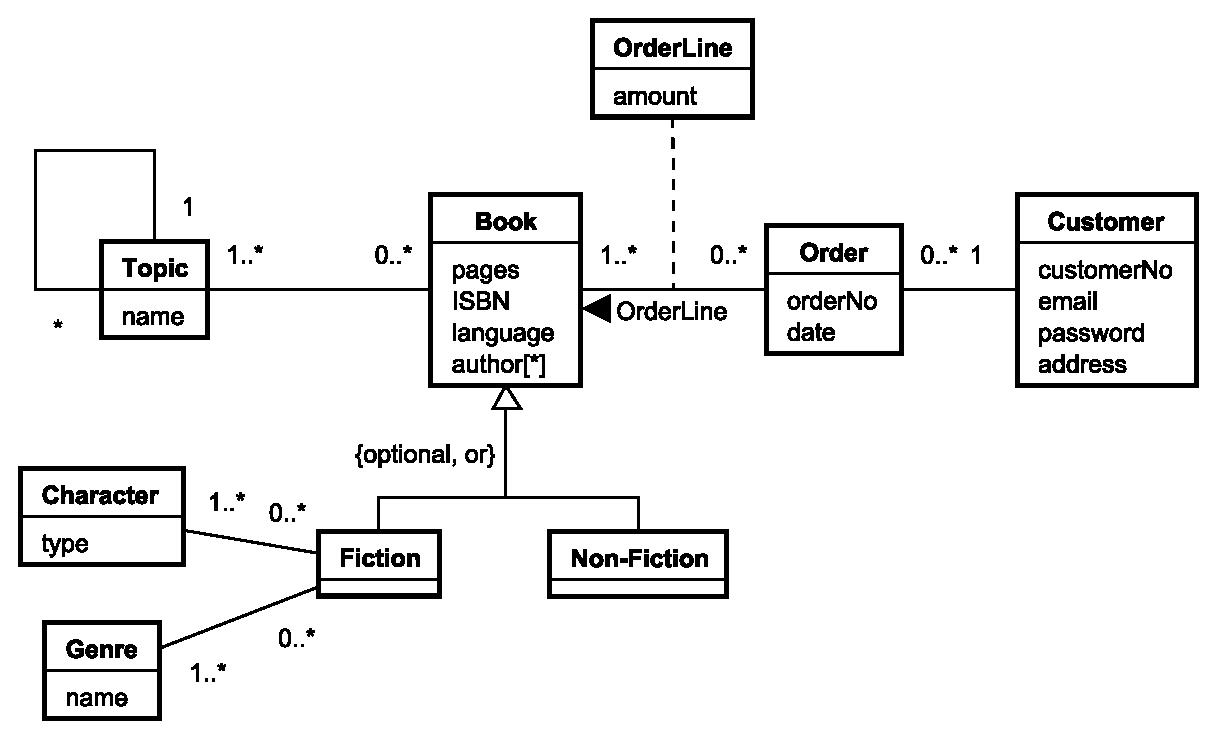
\includegraphics[width=\linewidth]{ConceptualModel.pdf}
		\caption{Conceptual Diagram}
		\label{fig:conceptual}
	\end{figure}
	\newline
	\subsection*{Decisions and Reasons}
	The first choice is deciding how Topic should handle the recursive relationship. The Parent Reference pattern is the simplest solution that helps in performing queries to find all topics. \newline
	The second choice is to remove entities, such as OrderLine, because they are no longer required to solve many to many relationships. They can be solved by storing an array of ids in one of the entities. All of these relationships are modelled in the same way. \newline
	The third choice is to have the following fields in book: type(Fiction, Non-Fiction), an array of objects for characters and an array to reference entries in genre. Genres are not book specific as most characters are. Books are genre specific, so the same genre appears frequently in many books. The array of objects for characters can work as long as there are not a lot of characters included. Usually it is important to have the few main characters that are specific to that book. This is the reason why characters are present in book. \newline
	The fourth choice is having authors just as an array of names. \newline
	The result is Fig \ref{fig:Mongo}. It describes the relationship between the collections in Mongo:
	\begin{figure}[h!]
		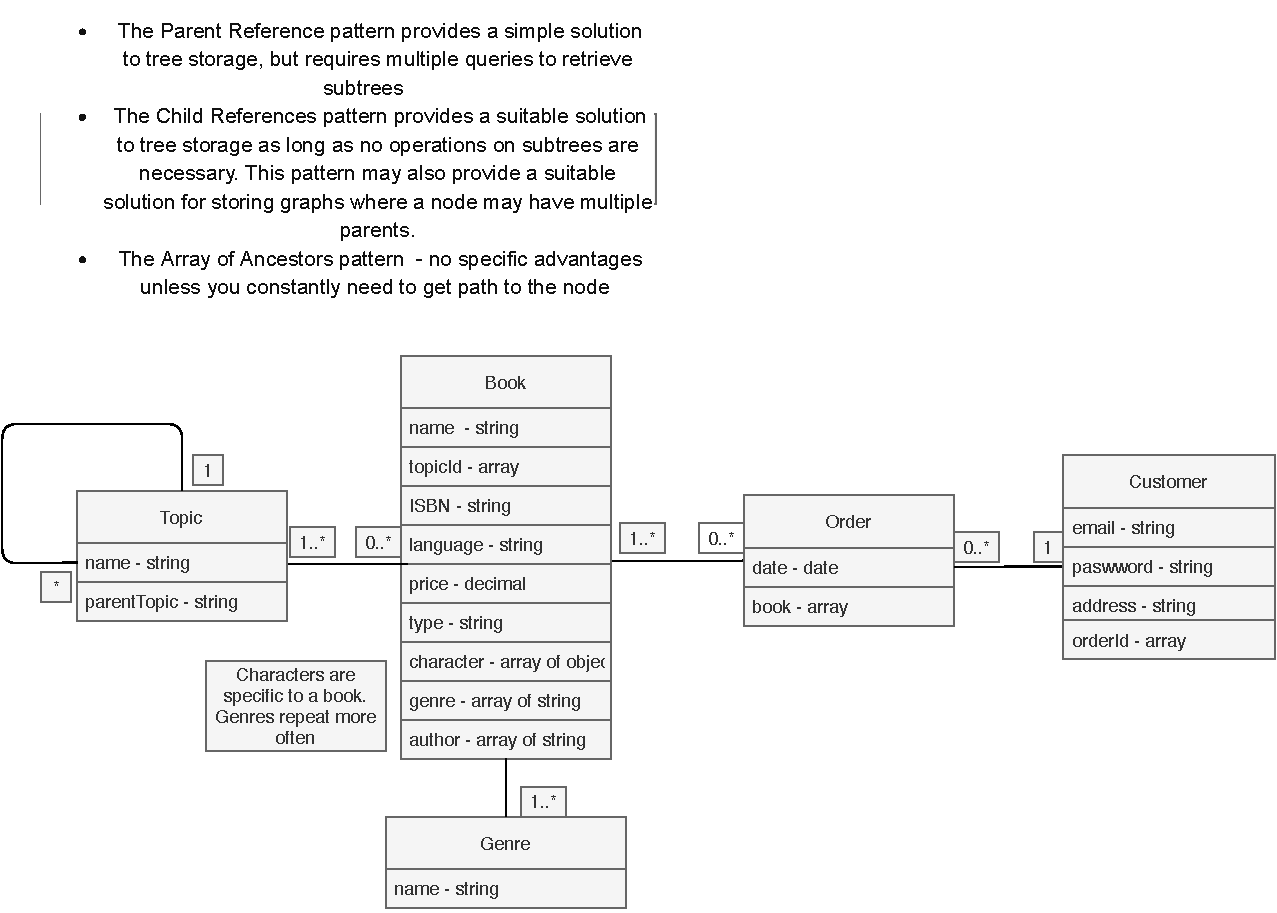
\includegraphics[width=\linewidth]{AmazonMongoDB.pdf}
		\caption{Amazon Books Mongo Diagram}
		\label{fig:Mongo}
	\end{figure}
	\subsection*{Consequences}
	A consequence of the first choice is the easiness of using graphLookup to find each topic.\newline 
	With the removal of entities that solves many to many cases, joining and performing different operations required more steps in the Mongo pipeline than it would otherwise in SQL. \newline
	Having type as a field instead of two different tables, while adding genre and characters when needed, makes it easy to handle the exercises in which it is mentioned. Less lookups are performed and the database is filled with less redundant data.\newline
	Usually, books don't have more than four authors, but one author can have many books. Having author just as an array of names makes it more taxing to perform queries, but it means less redundant data in the database. If more data is needed on an author than name, it can be a good idea to make it separate from book, but in this case it works well.
	\subsection*{The Exercises}
	The most difficult exercises are the ones that require to keep the values even though their aggregates are 0. For example, is it difficult to solve exercise nine because all books have to be in the response, even the ones that aren't being bought. Without this condition, the exercise is straight-forward. There are difficulties in making sure the syntax is correct. Even with simple use cases the queries can seem overwhelming.\newline
	Otherwise, most exercises are straightforward and the way pipelines work makes it easy to handle the documents. Each step of the pipeline makes logical sense due to the structure of documents being based on the idea of objects from object-oriented programming languages. Aggregating in Mongo is easier than in SQL, if the proper operators are known. The multitude of operators can get overwhelming, but for most cases, project, match and lookup are enough.\newline
	\subsection*{Comparison to Relational}
	Mongo is very flexible and leaves much of the design open to the context for which the database is built. With this said, it is harder to catch an error than it is usually in SQL. One of the main factors to this is the way references are handled. There isn't anything enforcing relationships, so an error can be introduced very easily, while being hard to detect. It is also easier to fix them than it would be in SQL, due to the flexibility. \newline
	The concept of json document makes it easier to design the collections and the relationships between them. Using tables in a SQL Database can seem unfamiliar because it requires a different mindset than the one used in programming. Mongo follows the mentality of object-oriented in comparison to SQL which leans more on set theory and logic. \newline
	
	\subsection*{Advantages and Disadvantages of Mongo in the Exercises}
	Advantages:
	\begin{enumerate}
		\item Flexibility
		\item Easier to understand as it focuses more on steps than nested queries
		\item Easier to fix errors
		\item Errors don't usually blow you up
	\end{enumerate}
	Disadvantages:
	\begin{enumerate}
		\item Syntax is overwhelming to write
		\item Cases in which aggregates are 0
		\item Easier to make errors
		\item Errors happen a lot more often
		\item Hard to ensure consistency
	\end{enumerate}
	\subsection*{Conclusion}
	In conclusion, Mongo seems better in situations in which strictness and consistency are not very important. It presents itself as very good in certain scenarios as IoT and similar fields in which it is hard to ensure that the correct data is sent through.
	
\end{document}